\chapter{APP AS A DATA ANALYSIS TOOL}
\label{chap:analysis_tool}

\textbf{Data analysis} is a procedure used to examine, clean, change and rebuild information with a view to reach to a specific decision for a given circumstance. Information investigation is normally of two sorts: subjective or quantitative. The sort of information directs the technique for examination. In subjective research, any non-numerical information like content or individual words are broke down. Quantitative examination, then again, centers around estimation of the information and can utilize insights to help uncover results and ends. The outcomes are numerical. At times, the two types of examination are utilized as an inseparable unit. For instance, quantitative investigation can help demonstrate subjective ends. \\

Spatial information investigation is concerned about that part of information examination where the land referencing of articles contains imperative data. This chapter talks about the ways this app can be used as an analysis tool directly or indirectly. \\

\section{Data downloading}

\textbf{Downloading} is defined as the transfer of data from server to your system or belonging. In other words, it is defined as the transmission of data from one machine to another. The significant advantage of downloading is that it gives you the full power over the information with the goal that you can utilize that information. \\

The app gives you the feature of exporting any admim level (0, 1 or 2) data in \gls{csv} format via email option so that it can be used in any form of spatial analysis.

Process of data downloading is described below.

\begin{itemize}
    \item Select year, date and tap on country to see the data and then tap on any region. Once you do that, you will see two buttons on both top corners of the screen. Figure 5.1 shows the two buttons which appears after having valid data on globe / map. \\
    
      \begin{figure}[H]
            \centering
            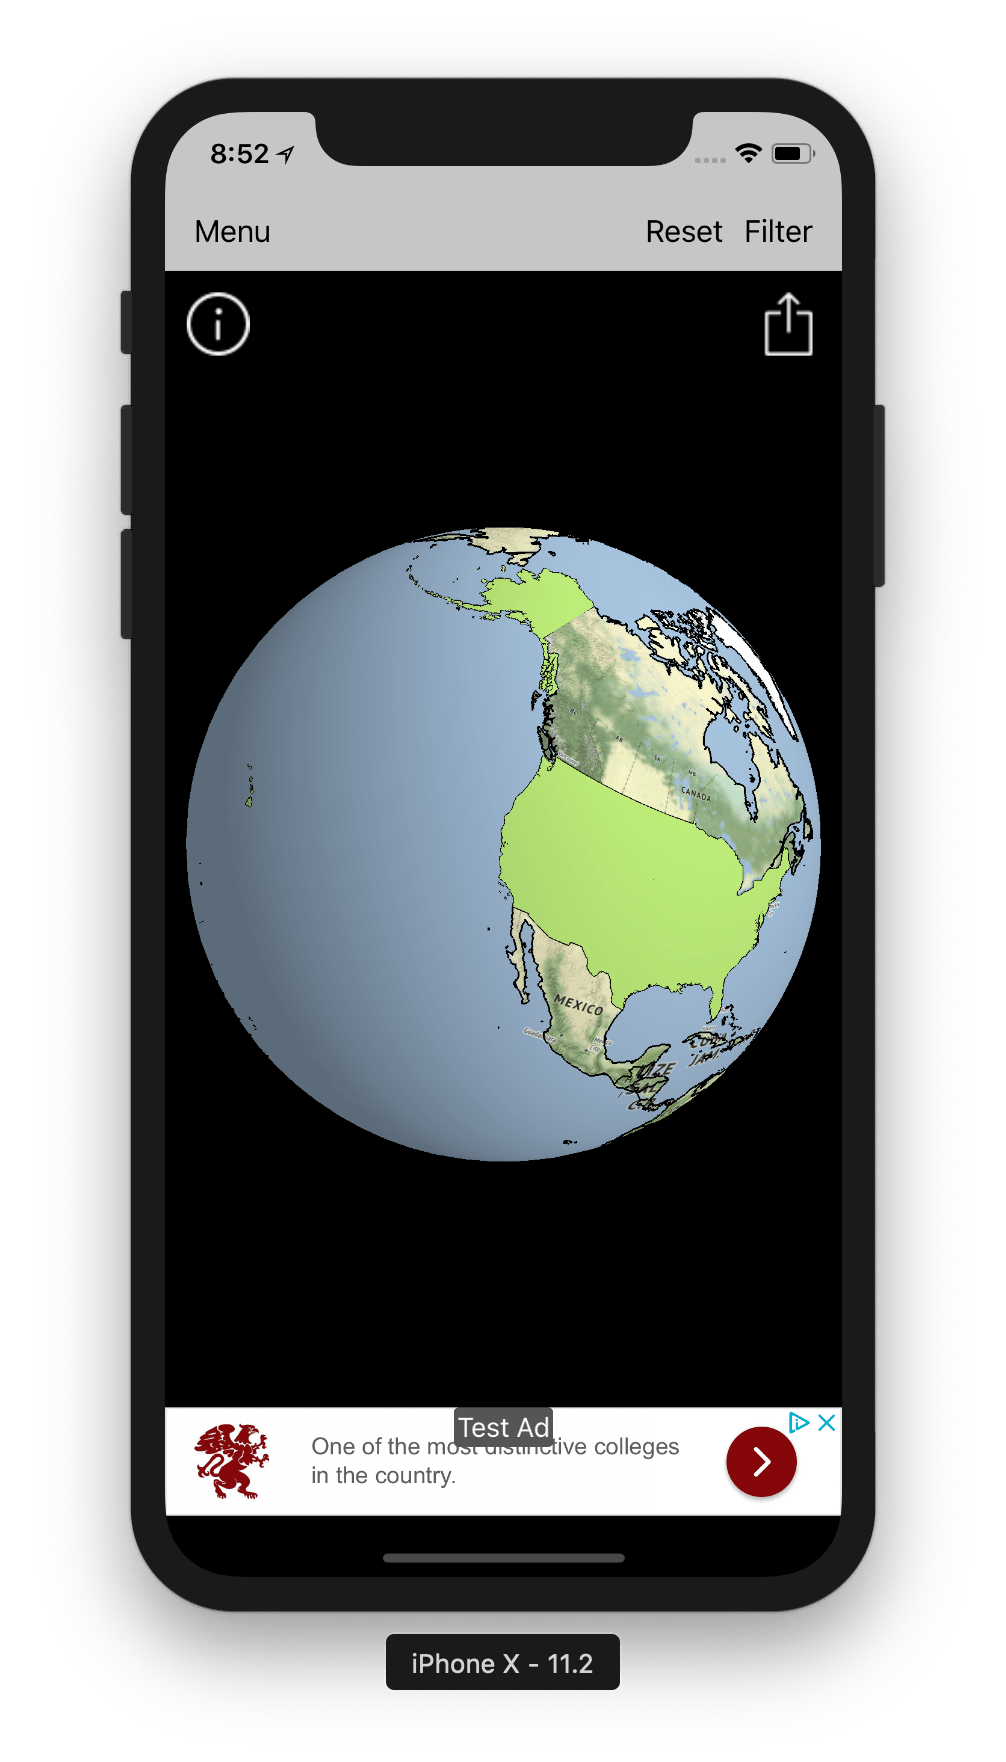
\includegraphics[width=0.25\linewidth]{figures/ch5/buttons.png}
            \caption{\label{fig:buttons} Home screen with two buttons on top corners}
        \end{figure}
     
    \item Left button in figure 5.1 corresponds to Info button which shows information about the current data that is being displayed. Figure 5.2 shows the view appears on tapping of information button. \\
    
      \begin{figure}[H]
            \centering
            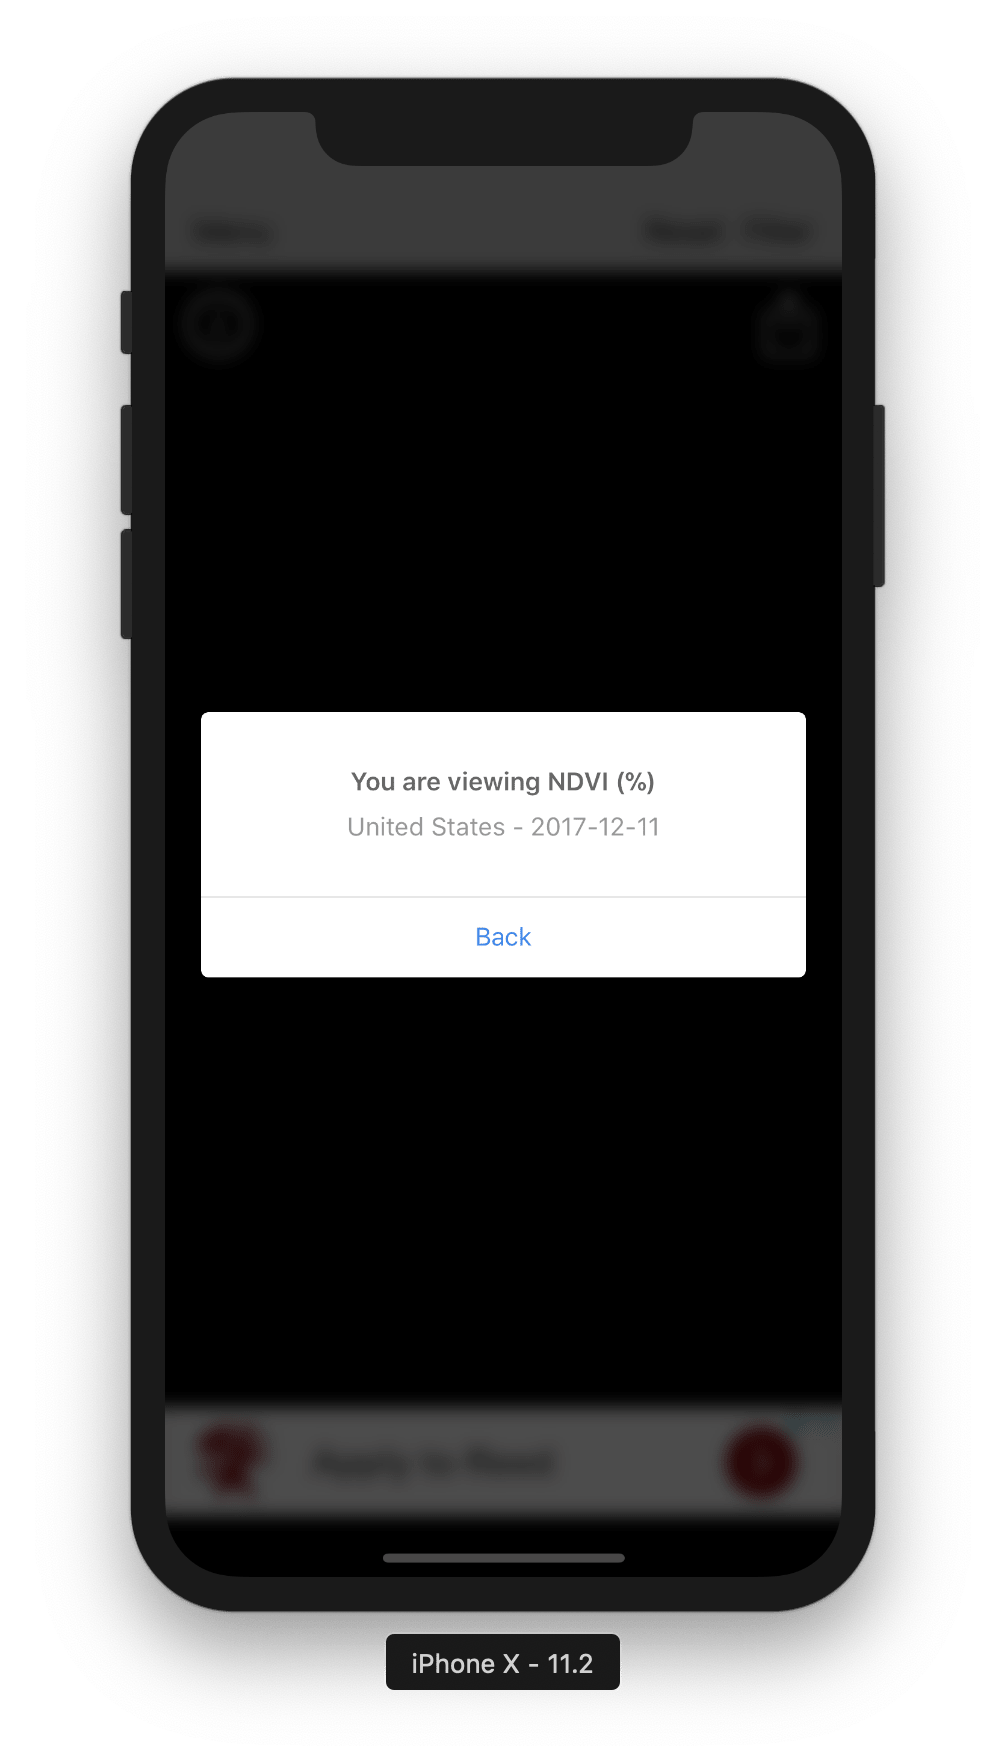
\includegraphics[width=0.25\linewidth]{figures/ch5/info_view.png}
            \caption{\label{fig:info_button} Information button action}
        \end{figure}
       
     \item Right button in figure 5.1 corresponds to export button which prompts you for exporting current data which is visible on globe / map. Figure 5.3 shows the export view on tapping of export button. \\
     
     \begin{figure}[H]
            \centering
            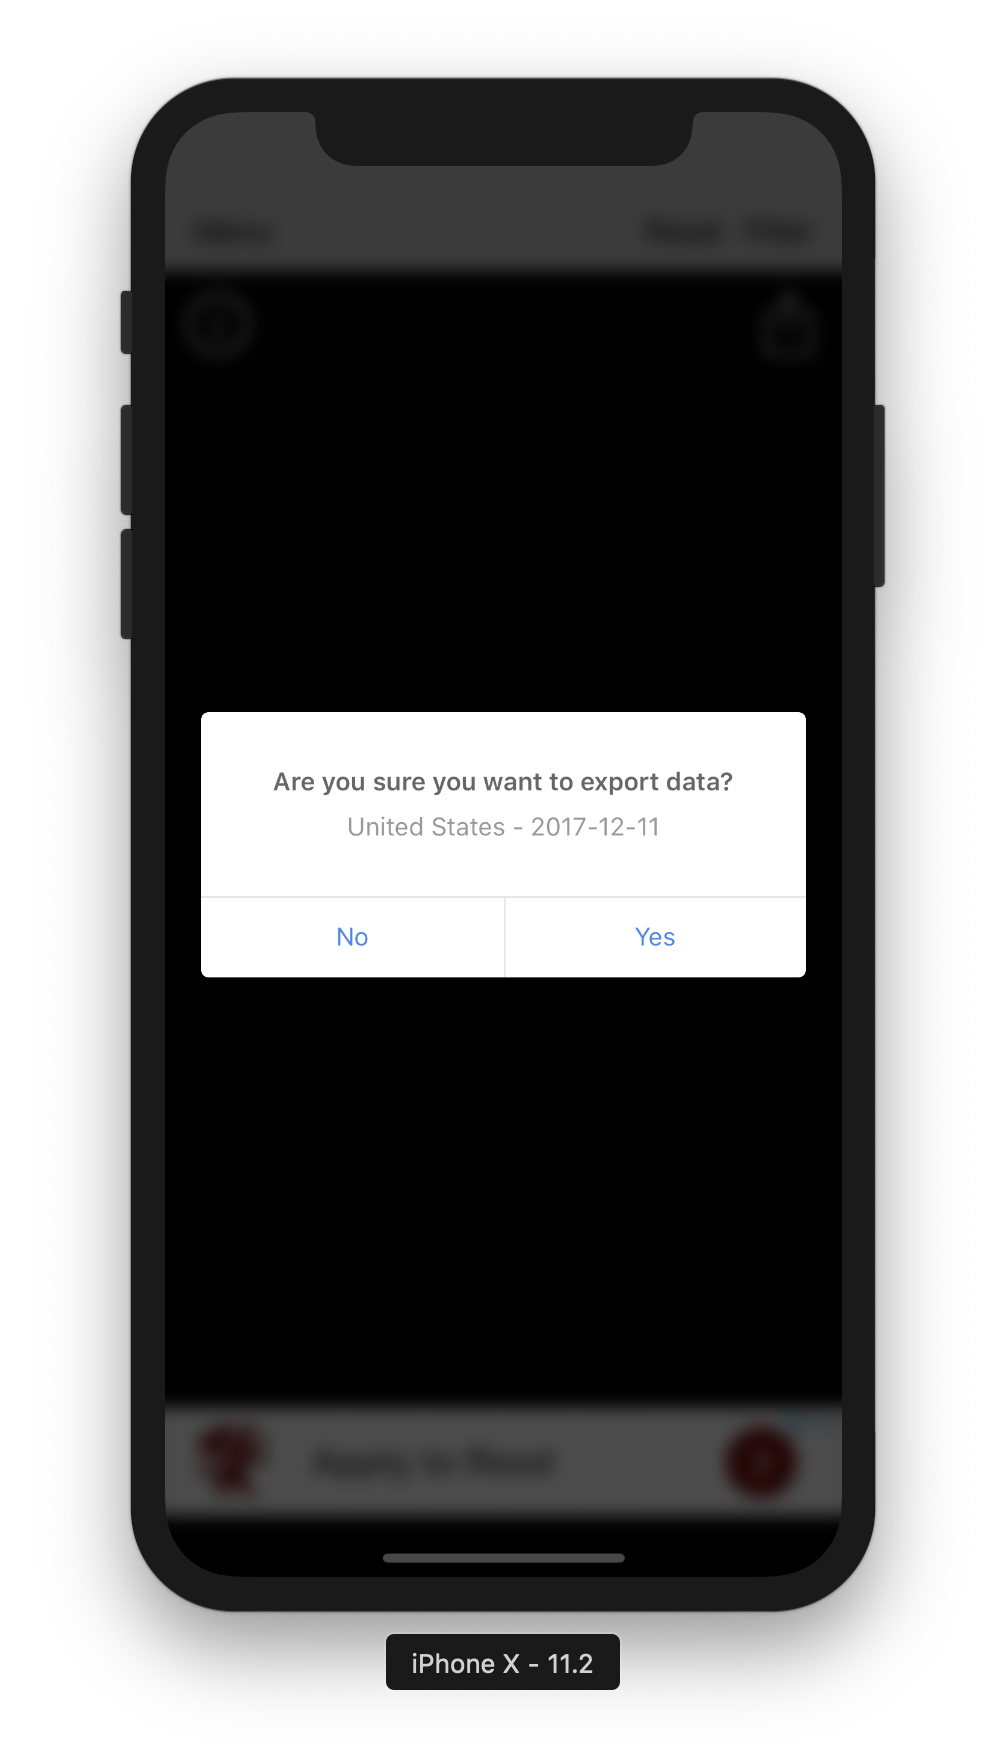
\includegraphics[width=0.25\linewidth]{figures/ch5/export_view.png}
            \caption{\label{fig:info_button} Export button action}
    \end{figure}
    
    On selecting yes in the figure 5.3, it then converts the raw \gls{json} data to a valid \gls{csv} format and attaches it as a file on the MFMailComposeViewController. \\
    
    %bibliography here add apple url link of definition
    
    According to Apple, It's a standard interface for managing, editing, and sending an email message in \gls{iOS} app. Figure 5.4 shows the MFMailComposerViewController view which helps user to email the \gls{csv} file.
    
    \begin{figure}[H]
            \centering
            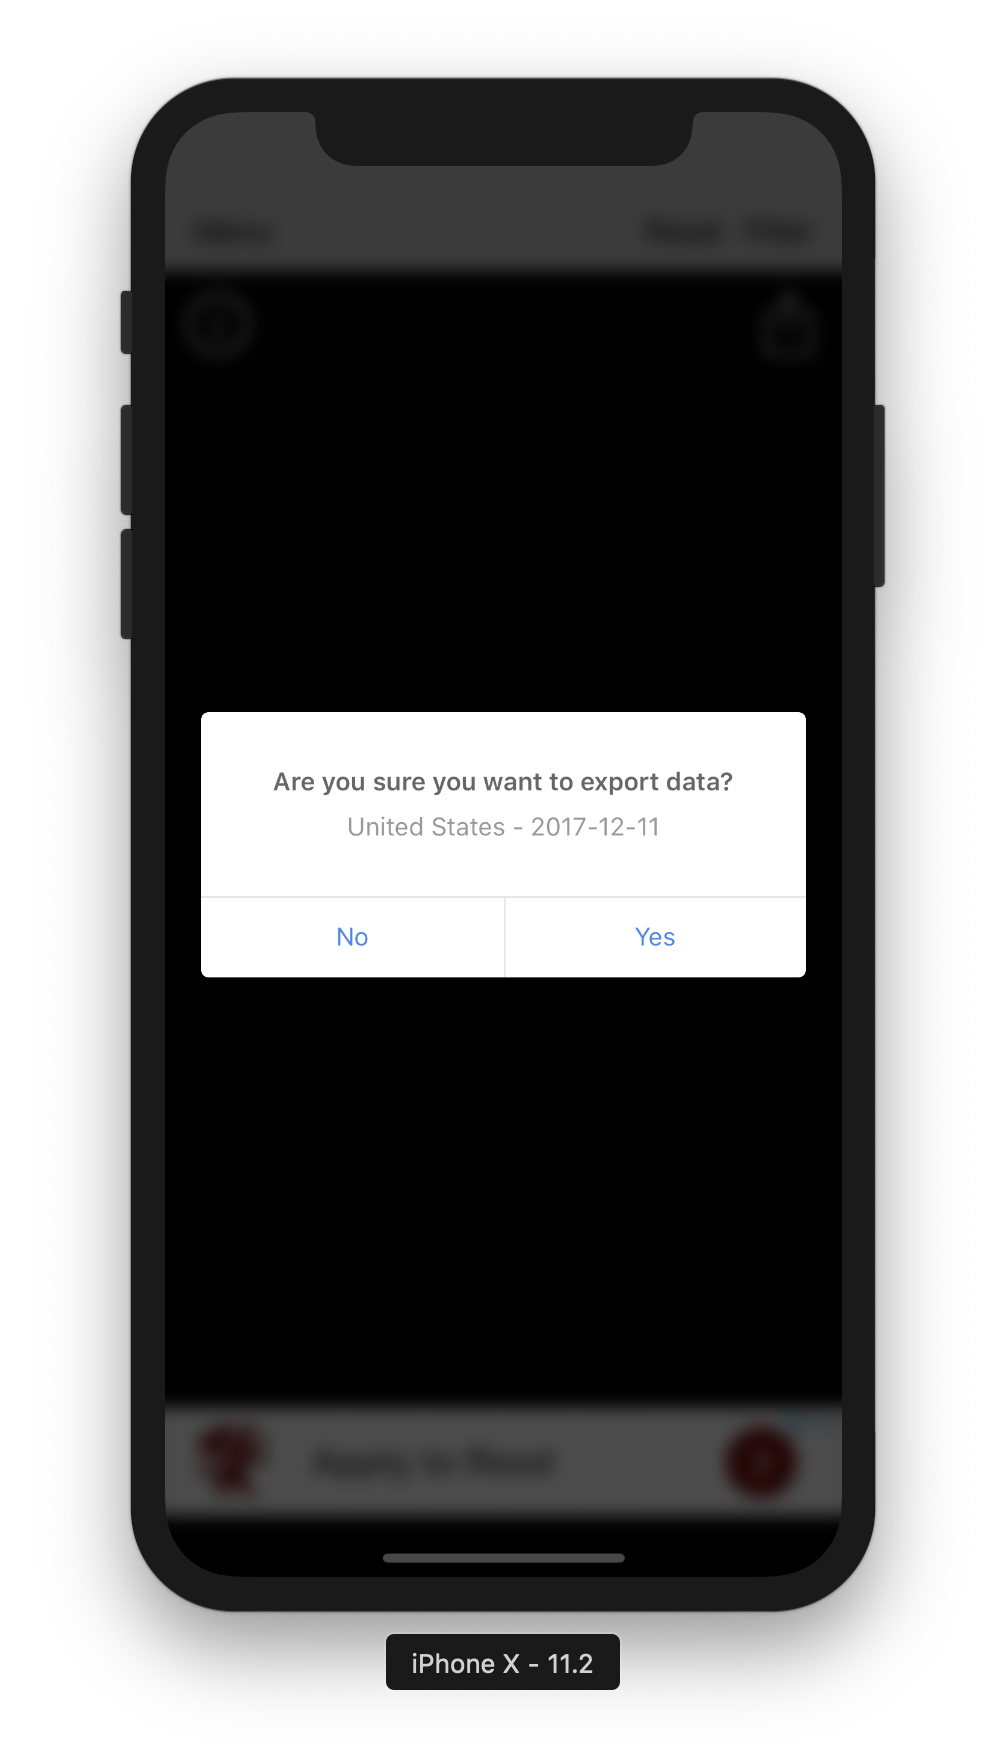
\includegraphics[width=0.25\linewidth]{figures/ch5/export_view.png}
            \caption{\label{fig:info_button} Export button action}
    \end{figure}
    
\end{itemize}

\section{Computing mean, Standard Deviation, histograms}

\section{SVD examples for patterns}


